\chapter{Calculo de ganancias para controladoers discontinuos homogeneos de grado cero} \label{Cap3}
\section{Controlador de primer orden}
Sea el sitema \ref{eq:modelo1} afin a la entrada, de grado relativo 1, 
\begin{subequations}\label{eq:modelo1}
  \begin{align}\label{eq:modelo1a}
    \dot{x}_1&=f(x) +u 
  \end{align}
\end{subequations}
Con el algoritmo de control discontinuo
  \begin{equation}
      u=-k_1 \left\lceil x_1  \right\rfloor^0
    \end{equation} 

    Función de Lyapunov de control
    \begin{equation}
          V_1=\gamma_1 \frac{r_1}{m} |x_1|^{\frac{m}{r_1}}
    \end{equation}
%%%%%%%%%%%%%%%%%%%%%%%%%%%%%%%%%%%%%%%%%%%%%%%%%%%%%%%5
%%%%5
%%%%%%%%%%%%%%%%%%%%%%%%%%%%%%%%%%%%%%%%%%%%%%%%%%%%%%%%%%
\section{Controlador de segundo orden}
Sea el sitema \ref{eq:modelo2} afin a la entrada, de grado relativo 2, 
\begin{subequations}\label{eq:modelo2}
  \begin{align}\label{eq:modelo1a}
    \dot{x}_1&=x_2 \\
    \dot{x}_2&=u
  \end{align}
\end{subequations}


  \begin{equation}
      \begin{split}
      \dot{x}_1&=x_2\\
      \dot{x}_2& \in [-C,C]+ [k_m, k_M] u
      \end{split}
      \label{inclusion2}
  \end{equation}
  Con el algoritmo de control discontinuo anidado
  \begin{equation}
      u=-k_2 \left\lceil \lceil x_2 \rfloor^{\alpha_2}+k_1^{\alpha_2} \lceil x_1 \rfloor^{\frac{\alpha_2}{2}} \right\rfloor^0
    \end{equation} 
    Función de Lyapunov de control
  \begin{equation}
        V_2=\gamma_1 \frac{r_1}{m} |x_1|^{\frac{m}{r_1}}+\frac{r_2}{m} |x_2|^{\frac{m}{r_2}}-\lceil \upsilon_1 \rfloor^{\frac{m-r_2}{r_2}} x_2 + \left(1-\frac{r_2}{m}\right)|\upsilon_1|^{\frac{m}{r_2}}
  \end{equation}
  \begin{equation}
        \upsilon_1=-k_1 \lceil x_1 \rfloor^{\frac{r_2}{r_1}}
   \end{equation}

   donde 
   \begin{equation}
        W_2 = \frac{r_2}{m} |x_2|^{\frac{m}{r_2}} - \lceil \upsilon_1 \rfloor^{\frac{m-r_2}{r_2}} x_2 + (1+\frac{r_2}{m})|\upsilon_1|^{\frac{m}{r_2}}
   \end{equation} 

   
   \begin{equation}
        \begin{split}
             \frac{\partial W_2}{\partial x_1}&=-\frac{m-r_2}{r_2} x_2 |\upsilon_1|^{\frac{m-2r_2}{r_2}} \frac{\partial \upsilon_1}{\partial x_1}+\frac{m-r_2}{r_2}\lceil \upsilon_1 \rfloor^{\frac{m-r_2}{r_2}}\frac{\partial \upsilon_1}{\partial x_1}\\
             &\textbf{sustituimos $x_2=s_2+\upsilon_1$} \\
             &=\frac{m-r_2}{r_2} \frac{\partial \upsilon_1}{\partial x_1} \left( -|\upsilon_1|^{\frac{m-2r_2}{r_2}}s_2 -\lceil \upsilon_1 \rfloor^{\frac{m-r_2}{r_2}} +\lceil \upsilon_1 \rfloor^{\frac{m-r_2}{r_2}} \right)\\
             &=-\frac{m-r_2}{r_2} \frac{\partial \upsilon_1}{\partial x_1} \left( |\upsilon_1|^{\frac{m-2r_2}{r_2}}s_2 \right)
        \end{split}
   \end{equation}

   donde
   \begin{equation}
       \upsilon_1=-k_1\lceil \sigma_1 \rfloor^{\frac{r_2}{\alpha_1}}=-k_1\lceil x_1 \rfloor^{\frac{r_2}{r_1}}
   \end{equation}
   \begin{equation}
       \frac{\partial \upsilon_1}{\partial x_1}= -k_1 \frac{r_2}{\alpha_1} |\sigma_1|^{\frac{r_2-\alpha_1}{\alpha_1}} \frac{\partial \sigma_1}{\partial x_1}  = -k_1 \frac{r_2}{r_1}|x_1|^{\frac{r_2-r_1}{r_1}}
   \end{equation}
   \begin{equation}
     \sigma_1=\lceil x_1 \rfloor^{\frac{\alpha_1}{r_1}}
   \end{equation}
   \begin{equation}
     \frac{\partial \sigma_1}{\partial x_1}=\frac{\alpha_1}{r_1} |x_1|^{\frac{\alpha_1-r_1}{r_1}}
   \end{equation}
   para llegar a la ecuacion del articulo tenemos
   \begin{equation}
     \frac{\partial \upsilon_1}{\partial x_1}= -k_1 \frac{r_2}{\alpha_1} |\sigma_1|^{\frac{r_2-\alpha_1}{\alpha_1}} \frac{\partial \sigma_1}{\partial x_1}= -k_1 \frac{r_2}{\alpha_1} \textcolor{red}{\frac{k_1^{\frac{r_2-\alpha_1}{r_2}}}{k_1^{\frac{r_2-\alpha_1}{r_2}}}}  |\sigma_1 |^{\textcolor{red}{\frac{r_2}{r_2}} \frac{r_2-\alpha_1}{\alpha_1}} \frac{\partial \sigma_1}{\partial x_1}
 \end{equation}
 \begin{equation}
   |\upsilon_1|^{\frac{r_2-\alpha_1}{r_2}}=|-k_1\lceil \sigma_1 \rfloor^{\frac{r_2}{\alpha_1}}|^{\frac{r_2-\alpha_1}{r_2}}=k_1^{\frac{r_2-\alpha_1}{r_2}}|\lceil \sigma_1 \rfloor^{\frac{r_2}{\alpha_1}}|^{\frac{r_2-\alpha_1}{r_2}}=k_1^{\frac{r_2-\alpha_1}{r_2}}|\sigma_1|^{\frac{r_2-\alpha_1}{\alpha_1}}
 \end{equation}
 
 por lo que 
 \begin{equation}
   \frac{\partial \upsilon_1}{\partial x_1}= -k_1 \frac{r_2}{\alpha_1} \textcolor{red}{\frac{1}{k_1^{\frac{r_2-\alpha_1}{r_2}}}} |\upsilon_1|^{\frac{r_2-\alpha_1}{r_2}} \frac{\partial \sigma_1}{\partial x_1}= -\frac{r_2}{\alpha_1} k_1^{\frac{\alpha_1}{r_2}} |\upsilon_1|^{\frac{r_2-\alpha_1}{r_2}} \frac{\partial \sigma_1}{\partial x_1}
\end{equation}
obtenemos la parcial de nuevo sustituyendo la ecuacion antetior
\begin{equation}
 \begin{split}
      \frac{\partial W_2}{\partial x_1}&=-\frac{m-r_2}{r_2} \frac{\partial \upsilon_1}{\partial x_1} \left( |\upsilon_1|^{\frac{m-2r_2}{r_2}}s_2 \right)\\
      &=-\frac{m-r_2}{r_2} \left(  -\frac{r_2}{\alpha_1} k_1^{\frac{\alpha_1}{r_2}} |\upsilon_1|^{\frac{r_2-\alpha_1}{r_2}} \frac{\partial \sigma_1}{\partial x_1} \right) \left( |\upsilon_1|^{\frac{m-2r_2}{r_2}}s_2 \right)\\
      &=\frac{m-r_2}{\alpha_1} k_1^{\frac{\alpha_1}{r_2}}  |\upsilon_1|^{\frac{m-r_2-\alpha_1}{r_2}}  s_2 \frac{\partial \sigma_1}{\partial x_1} \\
 \end{split}
\end{equation}

obtenemos la forma explicita de la parcial con respecto a $x_1$ de $W_2$
\begin{equation}
  \begin{split}
       \frac{\partial W_2}{\partial x_1}&=\frac{m-r_2}{\alpha_1} k_1^{\frac{\alpha_1}{r_2}}  |\upsilon_1|^{\frac{m-r_2-\alpha_1}{r_2}}  s_2 \frac{\partial \sigma_1}{\partial x_1} \\
       &=\frac{m-r_2}{\alpha_1} k_1^{\frac{\alpha_1}{r_2}}  |\upsilon_1|^{\frac{m-r_2-\alpha_1}{r_2}}  \left(x_2 -\upsilon_1 \right) \left(\frac{\alpha_1}{r_1} |x_1|^{\frac{\alpha_1-r_1}{r_1}}\right) \\
       &=\frac{m-r_2}{r_1} k_1^{\frac{\alpha_1}{r_2}}  |-k_1\lceil x_1 \rfloor^{\frac{r_2}{r_1}}|^{\frac{m-r_2-\alpha_1}{r_2}}  \left(x_2 +k_1\lceil x_1 \rfloor^{\frac{r_2}{r_1}} \right) \left( |x_1|^{\frac{\alpha_1-r_1}{r_1}}\right) \\
       &=\frac{m-r_2}{r_1} k_1^{\frac{m-r_2}{r_2}}  | x_1|^{\frac{m-r_2-\alpha_1}{r_1}}  \left(x_2 +k_1\lceil x_1 \rfloor^{\frac{r_2}{r_1}} \right) \left( |x_1|^{\frac{\alpha_1-r_1}{r_1}}\right) \\
       &=\frac{m-r_2}{r_1} k_1^{\frac{m-r_2}{r_2}}  | x_1|^{\frac{m-r_2-r_1}{r_1}}  \left(x_2 +k_1\lceil x_1 \rfloor^{\frac{r_2}{r_1}} \right) \\
  \end{split}
\end{equation}
llegando asi  a la expresion del articulo con la diferencia de no tener signo negativo


   Llamaremos $f_2$ a la función a maximizar
   \begin{equation*}
     k_2> \frac{1}{k_m}\left( max\left[f_2 \right] + C \right)
   \end{equation*}
   \begin{equation}
     %\begin{split}
       f_2(\overline{x}_2) =  \frac{x_2\left(\gamma_1 \lceil x_1 \rfloor^{\frac{m-r_1}{r_1}} + \frac{m-r_2}{r_1} k_1^{\frac{m-r_2}{r_2}}  | x_1|^{\frac{m-r_2-r_1}{r_1}}  \left(x_2 +k_1\lceil x_1 \rfloor^{\frac{r_2}{r_1}} \right) \right)} {\left|\lceil x_2 \rfloor^{\frac{m-r_2}{r_2}}+k_1^{\frac{m-r_2}{r_2}}\lceil x_1 \rfloor^{\frac{m-r_2}{r_1}}\right|}= \frac{\phi_2}{|s_{2d}|}
     %\end{split}    
   \end{equation}

   \begin{equation}
    \begin{split}
      \frac{\partial f_2}{\partial x_1}- \frac{\partial f_2}{\partial x_2}&=|s_{2d}|\left( \frac{\partial \phi_2}{\partial x_1}-\frac{\partial \phi_2}{\partial x_2}\right) + \phi_2\left(\frac{\partial |s_{2d}|}{\partial x_2}-\frac{\partial |s_{2d}|}{\partial x_1}\right)\\
      &=|s_{2d}|\left( \frac{\partial \phi_2}{\partial x_1}-\frac{\partial \phi_2}{\partial x_2}\right) + \phi_2 \frac{s_{2d}}{|s_{2d}|}  \left(\frac{\partial s_{2d}}{\partial x_2}-\frac{\partial s_{2d}}{\partial x_1}\right)  \\
      &=\textcolor{red}{|s_{2d}|} \left(  |s_{2d}|\left( \frac{\partial \phi_2}{\partial x_1}-\frac{\partial \phi_2}{\partial x_2}\right) + \phi_2 \frac{s_{2d}}{|s_{2d}|}  \left(\frac{\partial s_{2d}}{\partial x_2}-\frac{\partial s_{2d}}{\partial x_1}\right)\right)  \\
      &= |s_{2d}|^2\left( \frac{\partial \phi_2}{\partial x_1}-\frac{\partial \phi_2}{\partial x_2}\right) + \phi_2 s_{2d}  \left(\frac{\partial s_{2d}}{\partial x_2}-\frac{\partial s_{2d}}{\partial x_1}\right) \\
      &=\textcolor{red}{s_{2d}} \left(  s_{2d}\left( \frac{\partial \phi_2}{\partial x_1}-\frac{\partial \phi_2}{\partial x_2}\right) + \phi_2  \left(\frac{\partial s_{2d}}{\partial x_2}-\frac{\partial s_{2d}}{\partial x_1}\right)\right)  \\
    \end{split}
  \end{equation}
  en la ultima ecuacion podemos observar que $s_{2d}$ es una solución; sin embargo, corresponde a los puntos donde se va a menos infinito por lo que son puntos minimos y los descartamos.
   
   Como la función es homogénea de grado cero, obtendremos un rayo de máximos con la siguiente forma:\\
      con $\textcolor{red}{x_1=1}$

      \begin{equation}
       \begin{split}
         M_p&:= max\left[f_2 \right]= \left(  \frac{\partial \phi_2}{\partial x_2} -  \frac{\frac{\partial \phi_2}{\partial x_1}}{\frac{\partial s_{2d}}{\partial x_1}}  \frac{\partial s_{2d}}{\partial x_2} \right) =c + d x_2 - \left( \frac{a}{e}  x_2 + \frac{b}{e} x_2^2 \right) f  |x_2|^{\frac{m-2r_2}{r_2}} \\
       \end{split}
     \end{equation}

     donde las constantes que dependen del valor de $k_1$
     \begin{equation}
       a=\gamma_1 \frac{m-r_1}{r_1} +\frac{m-r_2}{r_1} \frac{m-r_1}{r_1} k_1^{\frac{m}{r_2}}  
     \end{equation}
     \begin{equation}
       b=\frac{m-r_2}{r_1} \frac{m-r_2-r_1}{r_1} k_1^{\frac{m-r_2}{r_2}}
     \end{equation}
     \begin{equation}
       c=\gamma_1 +\frac{m-r_2}{r_1}k_1^{\frac{m}{r_2}}
     \end{equation}
     \begin{equation}
       d=2\frac{m-r_2}{r_1} k_1^{\frac{m-r_2}{r_2}}
     \end{equation}
     \begin{equation}
       e=\frac{m-r_2}{r_1} k_1^{\frac{m-r_2}{r_2}}
     \end{equation}
     \begin{equation}
       f=\frac{m-r_2}{r_2}
     \end{equation}

     Para encontrar el valor del máximo se debe obtener una raíz del rayo de máximos y evaluar el punto en la función a maximizar $f_2$

     \begin{equation*}
       max= f(1,x_2)
     \end{equation*}

     Sustituyendo con los valores del caso mas sencillo:
      $m=3$,$ y_1=k_1=1$, $r=[2,1]$

      \begin{equation*}
       a=1;\;\;\;b=0;\;\;\;c=2;\;\;\;d=2;\;\;\;e=1;\;\;\;f=2;
      \end{equation*}
      con $x_2>0$
     \begin{equation}
       M_p=2+2x_2-2x_2^2
     \end{equation}

     \begin{equation}
       \textcolor{red}{x_2=-0.618};  \;\;\;\;  x_2=1.618
     \end{equation}


     El máximo se obtine al evaluar en la función original:
     \begin{equation}
       max=f_2(1,1.618)=1.618
     \end{equation}

     Por lo tanto $k_2>1.618$

      \begin{figure}
        \includegraphics[width=0.49\textwidth,]{imagenes/grado2/rayos}
        \includegraphics[width=0.49\textwidth,]{imagenes/grado2/parcialesMatalb.pdf}
        \caption{text}
        \label{text}
      \end{figure}
%%%%%%%%%%%%%%%%%%%%%%%%%%%%%%%%%%%%%%%%%%%%%%%%%%%%%%%%%%%%%%%%%%%%%%%%%%%%5
%%%%%%%%5      Grado 3
%%%%%%%%%%%%%%%%%%%%%%%%%%%%%%%%%%%%%%%%%5
\section{Para grado relativo 3}
Sea el sitema \ref{eq:modelo3} afin a la entrada, de grado relativo 3, 
\begin{subequations}\label{eq:modelo3}
  \begin{align}\label{eq:modelo1a}
    \dot{x}_1&=x_2 \\
    \dot{x}_2&=x_3 \\
    \dot{x}_3&=u
  \end{align}
\end{subequations}


  \begin{equation}
      \begin{split}
      \dot{x}_1&=x_2\\
      \dot{x}_2&=x_3\\
      \dot{x}_3& \in [-C,C]+ [k_m, k_M] u
      \end{split}
      \label{inclusion2}
  \end{equation}
  Con el algoritmo de control discontinuo anidado

    \begin{equation}
      u=-k_3 \left\lceil \lceil x_3 \rfloor^{\alpha_3}+k_2^{\alpha_3}\left\lceil \lceil x_2 \rfloor^{\frac{\alpha_2}{2}}+k_1^{\frac{\alpha_2}{2}} \lceil x_1 \rfloor^{\frac{\alpha_2}{3}}  \right\rfloor^{\frac{\alpha_3}{\alpha_2}} \right\rfloor^0
    \end{equation}
    
    Funcion de lyapunov de control
    \begin{equation}
      V_3=\gamma_2\left(\gamma_1 \frac{r_1}{m} |x_1|^{\frac{m}{r_1}}+\frac{r_2}{m} |x_2|^{\frac{m}{r_2}}-\lceil \upsilon_1 \rfloor^{\frac{m-r_2}{r_2}} x_2 + \left(1-\frac{r_2}{m}\right)|\upsilon_1|^{\frac{m}{r_2}}\right) +W_3
    \end{equation}

    La función a maximizar en su forma general:
    \begin{equation}
    k_2> max \left[ \frac{ \phi_2}{s_{2d} \lceil \sigma_2 \rfloor^{\frac{r_3}{\alpha_2}}} \right]:=max \left[ f_{32} \right]
  \end{equation}
Donde el rayo del máximo tiene la siguiente forma general:
  \begin{equation*}
    M:=\textcolor{red}{s_{2d} \frac{\partial \phi_2}{\partial x_1}- \phi_2 \left[ \frac{r_3}{\alpha_2} \frac{s_{2d} }{\sigma_2}  \frac{\partial \sigma_2}{\partial x_1} +  \frac{\partial s_{2d}}{\partial x_1}  \right]}
  \end{equation*}
Se fija $x_1=1$ y se busca una raiz para obtener el valor de $x_2$

\begin{equation}
  k_3> \frac{1}{k_m} max \left[  f_3 \right]+\frac{C}{k_m}:=\frac{1}{k_m}\frac{\phi_3}{|s_{3d}|}+\frac{C}{k_m}
\end{equation}
La función a obtener el máximo
\begin{equation}
  f_3:= \frac{\gamma_2 \gamma_1 x_2 s_{1d}   + \gamma_2  x_2  \frac{\partial W_2}{\partial x_1} + \gamma_2 x_3 \frac{\partial W_2}{\partial x_2}   + x_2 \frac{\partial W_3}{\partial x_1}  + x_3 \frac{\partial W_3}{\partial x_2}}{|s_{3d}|}
\end{equation}
Como la función es homogénea de grado cero, obtendremos un rayo de máximos con la siguiente forma:\\
con $\textcolor{red}{x_1=1, x_2=1}$
\begin{equation}
  \begin{split}
    max \left[  f_3 \right]=\frac{\partial \phi_3}{\partial x_3}- \frac{ \frac{\partial \phi_3}{\partial x_2}}{\frac{\partial s_{3d}}{\partial x_2}}\frac{\partial s_{3d}}{\partial x_3}=0\\
  \end{split}
\end{equation}



%%%%%%%%%%%%%%%%%%%%%%%%%%%%%%%%%%%%%%%%%%%%%%%%%%%%%%%%%%%%%%5
%%%          grado4
%%%%%%%%%%%%%%%%%%%%%%%%%%%%%%%%%%%%%%%%%%%%%%%%%%%%%%
\section{Para grado relativo 4}
Sea el sitema \ref{eq:modelo4} afin a la entrada, de grado relativo 4 , 
\begin{subequations}\label{eq:modelo4}
  \begin{align}\label{eq:modelo1a}
    \dot{x}_1&=x_2 \\
    \dot{x}_2&=x_3 \\
    \dot{x}_3&=x_4 \\
    \dot{x}_4&=u
  \end{align}
\end{subequations}


  \begin{equation}
      \begin{split}
      \dot{x}_1&=x_2\\
      \dot{x}_2&=x_3\\
      \dot{x}_3=x_4 \\
      \dot{x}_4& \in [-C,C]+ [k_m, k_M] u
      \end{split}
      \label{inclusion2}
  \end{equation}
  Con el algoritmo de control discontinuo anidado
  \begin{equation}
    u=-k_4 \left\lceil \lceil x_4 \rfloor^{\alpha_4}+ k_3^{\alpha_4} \left\lceil \lceil x_3 \rfloor^{\frac{\alpha_3}{2}}+k_2^{\frac{\alpha_3}{2}}\left\lceil \lceil x_2 \rfloor^{\frac{\alpha_2}{3}}+k_1^{\frac{\alpha_2}{3}} \lceil x_1 \rfloor^{\frac{\alpha_2}{4}}  \right\rfloor^{\frac{\alpha_3}{\alpha_2}} \right\rfloor^\frac{\alpha_3}{\alpha_2}\right\rfloor^0
  \end{equation}
  Función de Lyapunov de control
  \begin{equation}
    V_4=\gamma_3 V_3+W_4
  \end{equation}

  La función a maximizar en su forma general:
  \begin{equation}
  k_2> max \left[ \frac{ \phi_2}{s_{2d} \lceil \sigma_2 \rfloor^{\frac{r_3}{\alpha_2}}} \right]:=max \left[ f_{42} \right]
\end{equation}
Donde el rayo del máximo tiene la siguiente forma general:
\begin{equation*}
  M:=\textcolor{red}{s_{2d} \frac{\partial \phi_2}{\partial x_1}- \phi_2 \left[ \frac{r_3}{\alpha_2} \frac{s_{2d} }{\sigma_2}  \frac{\partial \sigma_2}{\partial x_1} +  \frac{\partial s_{2d}}{\partial x_1}  \right]}
\end{equation*}
Se fija $x_1=1$ y se busca una raiz para obtener el valor de $x_2$

La función a maximizar en su forma general:
\begin{equation}
k_3> max \left[ \frac{ \phi_3}{s_{3d} \lceil \sigma_3 \rfloor^{\frac{r_4}{\alpha_3}}} \right]:=max \left[ f_{43} \right]
\end{equation}
Donde el rayo del máximo tiene la siguiente forma general:
\begin{equation*}
M:=\textcolor{red}{s_{3d} \frac{\partial \phi_3}{\partial x_2}- \phi_3 \left[ \frac{r_4}{\alpha_3} \frac{s_{3d} }{\sigma_3}  \frac{\partial \sigma_3}{\partial x_2} +  \frac{\partial s_{3d}}{\partial x_2}  \right]}
\end{equation*}
Se fija $x_1=1, x_2=1$ y se busca una raiz para obtener el valor de $x_3$
\begin{equation}
  k_4> \frac{1}{k_m} max \left[  f_4 \right]+\frac{C}{k_m}:=\frac{1}{k_m}\frac{\phi_4}{|s_{4d}|}+\frac{C}{k_m}
\end{equation}
La función a obtener el máximo
\begin{equation}
  f_4:= \frac{ x_2 \frac{\partial V_4}{\partial x_1} + x_3 \frac{\partial V_4}{\partial x_2} + x_4 \frac{\partial V_4}{\partial x_3}  }{|s_{4d}|}
\end{equation}
Como la función es homogénea de grado cero, obtendremos un rayo de máximos con la siguiente forma:\\
con $\textcolor{red}{x_1=1, x_2=1, x_3=1}$
\begin{equation}
  \begin{split}
    max \left[  f_4 \right]=\frac{\partial \phi_4}{\partial x_4}- \frac{ \frac{\partial \phi_4}{\partial x_3}}{\frac{\partial s_{4d}}{\partial x_3}}\frac{\partial s_{4d}}{\partial x_4}=0\\
  \end{split}
\end{equation}

%%%%%%%%%%%%%%%%%%%%%%%%%%%%%%%%%%%%%%%%%%%%%%%%%%%%%%%%%%%%%%%%%%%%%%%%%%%%5
%%%%%%%%5      Grado 5
%%%%%%%%%%%%%%%%%%%%%%%%%%%%%%%%%%%%%%%%%5
\section{Para grado relativo 5}
Sea el sitema \ref{eq:modelo4} afin a la entrada, de grado relativo 4 , 
\begin{subequations}\label{eq:modelo4}
  \begin{align}\label{eq:modelo1a}
    \dot{x}_1&=x_2 \\
    \dot{x}_2&=x_3 \\
    \dot{x}_3&=x_4 \\
    \dot{x}_4&=x_5 \\
    \dot{x}_5&=u
  \end{align}
\end{subequations}


  \begin{equation}
      \begin{split}
        \dot{x}_1&=x_2 \\
        \dot{x}_2&=x_3 \\
        \dot{x}_3&=x_4 \\
        \dot{x}_4&=x_5 \\
      \dot{x}_5& \in [-C,C]+ [k_m, k_M] u
      \end{split}
      \label{inclusion2}
  \end{equation}
  Con el algoritmo de control discontinuo anidado
  \begin{equation}
    u=-k_5 \left\lceil \sigma_5 \right\rfloor^0
  \end{equation}
  \begin{equation}
    V_5=\gamma_4 V_4+W_5
  \end{equation}  
  
  %%%%%%%%%%%%%%%%%%%%%%%%%%%%%%%%%%%%%%%%%%%%%%%%%%%%%%%%%%%55
  %
  %%%%%%%%%
  %%%%%%%%%%%%%%%%%%%%%%%%%%%%%%%%%%%%%%%%%%%%%%%%%%%%%%%55
\section{Implementacion en Matlab}

%%%%%%%%%%%%%%%%%%%%%%%%%%%%%%%%%%%%%%%%%%%%%%%%%%%%%%%%%%%%%
%%
%%			Ejemplo empieza
%%
%%%%%%%%%%%%%%%%%%%%%%%%%%%%%%%%%%%%%%%%%%%%%%%%%%%%%%%%%%%%%%%
% In this chapter we present the first part of main result of this work. We introduce the design of Bl-homogeneous observers for SISO-LTI systems with bounded unknown inputs assuming strong observability. The idea is to transform the system in to a Special Coordinate Basis, (detailed in Chapter 2 for the MIMO general case) obtaining a representation of the system in which it is possible to design an UIO.

% Here we use directly a discontinuous nonlinear observer instead of differentiators. This fact suppress the necessity of using a cascade scheme composed by a linear observer and a discontinuous differentiator.

% The nonlinear injection terms can be designed to accelerate the convergence as much as we want by selecting appropriate and sufficiently large gains. Even more, due to the assignability of bl-homogeneous degrees in the observer we can reach and assure exact and finite-time (or moreover fixed-time) stability of the error estimation dynamics in presence of unknown inputs.
	
% \section{System transformation}
% Before attacking the MIMO case we will introduce the Single-Input Single-Output (SISO) case, which going to be useful in order to give the basic idea in solving the estimation problem.

% Consider the SISO-LTI system without feedthrough (for simplicity) given by
% \begin{equation}
% 	\begin{split}\label{ecu: Sys siso orig}
% 	\Sigma: \left\{
% 	\begin{array}{rl}
% 		\dot{x} &= Ax + D\omega\\
% 		y&=Cx
% 	\end{array}
% 	\right. \\
% 	\end{split}
% \end{equation}
% where $x \in \RE^n$ is the state vector, $\omega \in \RE$ the unknown input and $y \in \RE$ is the output of the system. Accordingly, the matrices $A,D,C$ have appropriate dimensions. For simplicity in the development we do not consider a known input $u$, since it does not modify the observability properties and it is simple to include it in the observer design. 

% The task is to build an observer providing for finite-time (preferably fixed-time convergent and exact) estimation of the states in presence of the unknown input. In the previous chapters we have stated the general conditions for the existence and characterization of unknown input observers (UIO). Here we will recall this conditions in the particular case we are working on.

% The equations in the observer will be understood in the Filippov sense \cite{Filippov1988} in order to provide for the possibility to use discontinuous signals. Note that Filippov solutions coincide with the usual solutions, when the right-hand sides are continuous.

% Accordingly to the Definitions \ref{def: CH2 Rosenbrok} and \ref{def: CH2 Strongly obs} the system \eqref{ecu: Sys siso orig} is strongly observable if the triple ($A,D,C$) has no invariant zeros. Unfortunately, this definition does not give specific nor convenient form to the system matrices. Special Coordinate Basis for SISO case (a particular case of MIMO-SCB presented in Chapter 2) clarifies this problem.

% \begin{theorem}\label{theo: SCB SISO}
% 	Consider the system \eqref{ecu: Sys siso orig}. There exist nonsingular state, input and output transformations $\Gamma_s\in \RE^{n\times n},\Gamma_i\in \RE,\Gamma_o\in \RE$, which decompose the state space of $\Sigma$ into two subspaces, $x_a$ and $x_d$. These two subspaces correspond to the finite zero and infinite zero structures of $\Sigma$, respectively. The new state space, input and output spaces of the decomposed system are described by the following set of equations:
	
% 	\begin{equation}\label{ecu: CH3 Transf SCB SISO}
% 		x=\Gamma_s\bar{x}, \quad y=\Gamma_o\bar{y}, \quad u=\Gamma_i\bar{u},
% 	\end{equation}
% 	\begin{equation}
% 		\bar{x}=
% 		\begin{bmatrix}
% 			x_a \\
% 			x_d
% 		\end{bmatrix}, x_a \in \mathbb{R}^{n_a}, \quad x_d \in \mathbb{R}^{n_d},\quad x_d=
% 		\begin{bmatrix}
% 			x_{d,1} \\
% 			x_{d,2} \\
% 			\vdots \\
% 			x_{d,n_d}
% 		\end{bmatrix},
% 	\end{equation}
% 	and
% 	\begin{equation}
% 		\begin{split}\label{ecu: CH3 SISO SCB sys}
% 		\Sigma_{SCB}: \left\{
% 			\begin{array}{rl}
% 			\dot{x}_a &= A_{aa}x_a + H_{ad}y\\
% 			\dot{x}_{d,1} &= x_{d,2}, \quad y=x_{d,1}, \\
% 			\dot{x}_{d,j} &= x_{d,j+1} \\
% 			& \vdots \quad j=2,...,n_{d}-1\\
% 			\dot{x}_{d,n_{b}} &= a_{d,1}x_{d,1} + a_{d,2}x_{d,2} +...+ a_{d,n_d}x_{d,n_d} + \omega
% 			\end{array}
% 		\right. \\
% 		\end{split}
% 	\end{equation}
% \end{theorem}

% Similar to Property \ref{prop: CH2 SCB strong obsv} we have:
% \begin{property}\label{prop: CH3 S observability}
% 	The system $\Sigma_{SCB}$ in \eqref{ecu: CH3 SISO SCB sys} is strongly observable if and only if $x_a$ is non-existent.
% \end{property}

% %Another characterization for strongly observable LTI systems in terms of the relative degree with respect to the unknown input was introduced in \cite{Fridman2006}.
% %
% %\begin{definition}
% %	Following \cite{Isidori1996} the relative degree of system \eqref{ecu: Sys siso orig} with respect to the unknown input is the number $r$ such that
% %	\begin{equation}
% %		CA^jD=0. \quad j=1,...,r-2, \quad CA^{r-1}D \neq 0
% %	\end{equation}
% %\end{definition}
% %Since the system \eqref{ecu: Sys siso orig} is assumed to be observable (in absence of unknown input), i.e. the matrix 
% %
% %\begin{equation}
% %	\mathcal{O} = \begin{bmatrix}
% %		C \\
% %		CA \\
% %		\vdots \\
% %		CA^{n-1}
% %	\end{bmatrix}
% %\end{equation}
% %
% %has full rank. Then we can transform the system to the observability canonical form through the state transformation $T=\mathcal{O}^{-1}$, such that the matrices $A,D,C$ take the form

% This is equivalent to have relative degree $n$ with respect to the unknown input $\omega(t)$. This latter is a sufficient condition of strong observability presented in \cite{Fridman2006}. 

% If we assume strong observability, then we can apply an extra transformation $\Gamma_{\mathcal{O}}=\mathcal{O}^{-1}$, where $\mathcal{O}$ is the observability matrix and transforms the system in observability canonical form.

% \section{Unknown Input Observer design}
% Given a strongly observable system $\Sigma$ in \eqref{ecu: Sys siso orig} under the SCB transformation \eqref{ecu: CH3 Transf SCB SISO}, and suppressing the subscript $d$ for simplicity in notation, the system is given by
% \begin{equation}
% 	\begin{split}\label{ecu: SISO SCB sys SO}
% 		\Sigma_s: \left\{
% 		\begin{array}{rl}
% 		\dot{x}_{1} &= x_{2}, \quad y=x_{1}, \\
% 		\dot{x}_{j} &= x_{j+1} \\
% 		& \vdots \quad j=2,...,n_{d}-1\\
% 		\dot{x}_{n} &= A_{dd}x + \omega, 
% 		\end{array}
% 		\right. \\
% 	\end{split}
% \end{equation}
% where $A_{dd}= \begin{bmatrix}  a_{1} & a_{2} & \hdots & a_{n} \end{bmatrix}$ and we have by Property \ref{prop: CH3 S observability} that $n_d=n$ and it is assumed the following.
% \begin{assumtion}\label{Assum: omega}
% 	Unknown input $\omega(t)$ a is uniformly bounded function, $|\omega(t)|\leq \Delta, \quad \Delta \in \RE_{\geq 0}$
% \end{assumtion}
% This allow us to relax the existence conditions of UIO's in o order to have an observer under strong observability only, see Section 2.2. It has to be noted that the system \eqref{ecu: SISO SCB sys SO} is in the observability canonical form, which requires the bl-homogeneity of the observer, since the observer canonical form can be implemented with a homogeneous differentiator (as already done in \cite{Niederwieser2021}). It is clear that in observer form the bl-homogeneous observer can also be implemented.

% The observer is given by
% \begin{equation}\label{ecu: Obs SISO}
% 	\begin{split}
% 	\Omega: \left\{
% 	\begin{array}{rl}
% 		\dot{\hat{x}}_{1} &= -k_{1}L \tilde{\phi}_{1}( \hat{x}_{1}-y ) + \hat{x}_2 \\
% 		\dot{\hat{x}}_{j} &= -k_{j}L^{j}\tilde{\phi}_{j}( \hat{x}_{1}-y ) + \hat{x}_{j+1} \\
% 		\vdots \quad & j=2,...,n-1\\
% 		\dot{\hat{x}}_{n} &= -k_{n}L^{n} \tilde{\phi}_{n}( \hat{x}_{1}-y ) + A_{dd}\hat{x}
% 	\end{array}
% 	\right. \\
% 	\end{split}
% \end{equation}
% with positive external gains $k_j>0$ and positive tuning gains $\alpha,L >0$, appropriately selected as it will be show latter. The output injection terms $\tilde{\phi}_{j}(\cdot)$ are obtained from the functions

% \begin{equation}\label{ecu: Injection SISO}
% 	\phi_{j}(s) = \kappa_{ j} \sig{ s }{\frac{r_{0,j+1}}{r_{0,1}}} + \theta_{ j} \sig{ s }{\frac{r_{\infty,j+1}}{r_{\infty,1}}}
% \end{equation}

% by scaling the positive internal gains $\kappa_{ j}>0,\theta_{ j}>0$
% \begin{equation}
% 	\kappa_{ j} \rightarrow \left( \frac{L^{n}}{\alpha}\right)^{\frac{jd_0}{r_{0,1}}}\kappa_{ j} ,\qquad \theta_{ j} \rightarrow \left( \frac{L^{n}}{\alpha}\right)^{\frac{jd_{\infty}}{r_{\infty,1}}}\theta_{ j}
% \end{equation}

% with powers selected as $r_{0,n}=r_{\infty,n}=1$, and
% \begin{equation}\label{ecu: r-siso}
% 	\begin{split}
% 		r_{0,j} = r_{0,j+1}-d_0 = 1-(n-j)d_0 \\
% 		r_{\infty,j} = r_{\infty,j+1}-d_{\infty} = 1-(n-j)d_{\infty}
% 	\end{split}
% \end{equation}
% which are completely defined by two parameters $d_0,d_{\infty}$. They have to satisfy $-1\leq d_0 \leq d_{\infty} < \frac{1}{n-1}$.

% We have to highlight the fact that injection terms in \eqref{ecu: Obs SISO} and \eqref{ecu: Injection SISO} are very similar to them in the bl-homogeneous differentiator \eqref{ecu: dif Mor} but the ones here are simpler. This simplifies the task of implementation. 

% \subsection{Gain Selection}
% 	Each type of gain in the observer has a different role, and the idea in the gain tuning is very intuitive.
% 	\begin{enumerate}
% 		\item The internal gains $\kappa_j > 0, \theta_j > 0$ can be selected arbitrary. They can be selected as arbitrary positive real values, and correspond to the desired weighting of each term of low degree and high degree respectively in $\phi_j$.
% 		\item The external gains $k_j > 0$ have the objective of stabilizing the observer in absence of interconnections and external perturbations, i.e. when $A_{dd}=0$ and $\omega(t)=0$.
% 		\item Parameter $L$ is selected large enough to assure the convergence in presence of interconnections, but not of the bounded
% 		perturbations $\omega(t)$. Setting its value greater than minimal value to assure stability the convergence velocity will be increased.
% 		\item The tuning parameter $\alpha$ is selected large enough to assure the convergence in presence of the bounded unknown input $\omega(t)$.
% 	\end{enumerate}

% \subsection{Estimation in original coordinates}
% The estimated state obtained from the observer $\Omega$ in \eqref{ecu: Obs SISO} corresponds to the transformed system $\Sigma_{SCB}$ in \eqref{ecu: SISO SCB sys SO} represented in SCB coordinates through the state $\Gamma_s$, input $\Gamma_i$ and output $\Gamma_o$ transformations \eqref{ecu: CH3 Transf SCB SISO}, moreover it was applied an extra transformation $\Gamma_{\mathcal{O}}=\mathcal{O}^{-1}$ which puts the system in observability canonical form. 

% The states in original coordinates can be computed as
% \begin{equation}\label{ecu: CH3 invers transf}
% 	x = \Gamma_s\Gamma_{\mathcal{O}}\hat{x}
% \end{equation}

% Therefore, the observer in original coordinates for the system \eqref{ecu: Sys siso orig} takes the form

% \begin{equation}\label{ecu: CH3 Observer Orig Coord}
% 	\begin{split}
% 		\dot{\hat{x}} &= -\Gamma_s\Gamma_{\mathcal{O}} K\Phi(e_y) + A\hat{x} + Bu \\
% 		e_y &= \Gamma_o^{-1}(\hat{y}-y)\\
% 		\hat{y} &= C\hat{x}
% 	\end{split}
% \end{equation}
% with
% \begin{equation}\label{ecu: CH3 Observer Orig Coord param}
% 	\begin{split}
% 		K &= \text{diag}(k_1L,k_2L^2,...,k_nL^n)\\
% 		\Phi(\hat{y}-y) &=
% 		\begin{bmatrix}
% 			\tilde{\phi}_{1}( e_y ) & \tilde{\phi}_{2}( e_y ) & ,\hdots, & \tilde{\phi}_{n}( e_y )
% 		\end{bmatrix}^T
% 	\end{split}
% \end{equation}

% \subsection{Main result. UIO - SISO case}
% The main result of this work in the SISO case establishes that the Unknown Input Observer \eqref{ecu: Obs SISO} is able to estimate at least asymptotically the states of a strongly observable linear system.

% \begin{theorem}\label{theo: CH3 Obsv SISO}
% 	Let the strongly observable SISO-LTI system $\Sigma$ \eqref{ecu: Sys siso orig} has an UIO given by \eqref{ecu: CH3 Observer Orig Coord},\eqref{ecu: CH3 Observer Orig Coord param}. Select $-1\leq d_0\leq d_{\infty}<\frac{1}{n-1}$ and chose arbitrary (internal gains)  $\kappa_j>0$ and $\theta_j>0$, for $j=1,...,n$. Suppose that either $\Delta=0$ or $d_0=-1$. Under this conditions,  there exist appropriate gains $k_j>0$, for $j=1,...,n$, and parameters $L>0,\alpha>0$ sufficiently large such that the solutions of bl-homogeneous UIO \eqref{ecu: Obs SISO} converge globally and asymptotically to the true states of $\Sigma_s$, i.e. $\hat{x}_j(t) \rightarrow x_j(t)$ as $t \rightarrow \infty$.
	
% 	In particular, it can converge globally and %in Fixed-Time if either
% %	\begin{itemize}
% %		\item exponentially if $d_0=0$ with $\Delta=0$,
% %		\item finite-time if  $d_0 < 0$ with $\Delta=0$ or $d_0=-1$ with $\Delta\neq 0$
% %		\item fixed-time if $d_0<0$ and $d_{\infty}>0$ subject to
% %		\begin{eqnarray*}
% %			&(a)& \quad -1 < d_0 < 0 < d_\infty < \tfrac{1}{n-1} \quad \text{with} \quad \Delta \equiv 0,  \quad or \\
% %			&(b)& \quad -1 = d_0 < 0 < d_\infty < \tfrac{1}{n-1} \quad \text{with} \quad \Delta \neq 0.
% %		\end{eqnarray*}
% %	\end{itemize}
% 	\begin{itemize}
% 			\item exponentially if
% 			\begin{equation}
% 				 d_0=0 \quad\text{with}\quad \Delta \equiv 0,
% 			\end{equation}
% 			\item finite-time if 
% 			\begin{equation}
% 				\begin{split}
% 				&(a) \quad -1 < d_0 < 0 \quad\text{with}\quad \Delta \equiv 0, \quad or  \\
% 				&(b) \quad d_0 =-1 \quad\text{with}\quad \Delta\neq 0
% 				\end{split}
% 			\end{equation}
% 			\item fixed-time if
% 			\begin{equation}
% 				\begin{split}
% 				&(a) \quad -1 < d_0 < 0 < d_\infty < \tfrac{1}{n-1} \quad \text{with} \quad \Delta \equiv 0,  \quad or \\
% 				&(b) \quad -1 = d_0 < 0 < d_\infty < \tfrac{1}{n-1} \quad \text{with} \quad \Delta \neq 0.
% 				\end{split}
% 			\end{equation}
% 		\end{itemize}
% \end{theorem}

% \subsection[Proof]{Proof of Theorem \ref{theo: CH3 Obsv SISO}}  
% 	The proof will be carried out in a Lyapunov framework through a bl-homogeneous Lyapunov function, this one can be used to realize an estimation fo the convergence time and calculation of gains $k_j$ moreover in an optimal sense. Part of this work had been presented in \cite{Moreno2021}. This work does not address the problem.

% 	To study the error system in a more suitable form, we are going to take the system and observer in the transformed SCB coordinates, i.e. the system \eqref{ecu: SISO SCB sys SO}	and observer \eqref{ecu: Obs SISO}. It is clear that the analysis is completely equivalent in original coordinates.
	
% 	Let the estimation error $e_j = \hat{x}_j - x_j$. The dynamics error are described by
% 	\begin{equation}\label{ecu: Error SISO 1}
% 		\begin{split}
% 			\Xi: \left\{
% 			\begin{array}{rl}
% 				\dot{e}_{1} &= -k_{1}L \tilde{\phi}_{1}( e_1 ) + e_2 \\
% 				\dot{e}_{j} &= -k_{j}L^{j}\tilde{\phi}_{j}( e_1 ) + e_{j+1} \\
% 				\vdots \quad & j=2,...,n-1\\
% 				\dot{e}_{n} &= -k_{n}L^{n} \tilde{\phi}_{n}( e_1 ) + A_{dd}e - \omega
% 			\end{array}
% 			\right. \\
% 		\end{split}
% 	\end{equation}
% 	where, by Assumption \ref{Assum: omega} $\omega(t)\leq\Delta$. Applying the time scaling via the next transformation
	
% 	\begin{equation}
% 		\epsilon_{j}=\frac{L^{{n}-j+1}}{\alpha}e_{j},\quad j=1,...,n
% 	\end{equation}
% 	we obtain 
% 	\begin{equation}\label{ecu: Error SISO 2}
% 		\begin{split}
% 			\Xi^{\star}: \left\{
% 			\begin{array}{rl}
% 				\dot{\epsilon}_{1} &= L\left[ -k_{1} \phi_{1}( \epsilon_{1} ) + \epsilon_{2} \right] \\
% 				\dot{\epsilon}_{j} &= L\left[ -k_{j} \phi_{j}( \epsilon_{1} ) + \epsilon_{j+1} \right] \\
% 				\vdots \quad & j=2,...,n-1\\
% 				\dot{\epsilon}_{n} &= L\left[ -k_{n} \phi_{n}( \epsilon_{1} ) + \frac{1}{\alpha}\Psi_{i}(\epsilon,\omega) \right]
% 			\end{array}
% 			\right. \\
% 		\end{split}
% 	\end{equation}
% 	where
% 	\begin{equation}\label{ecu: Psi 1}
% 		\begin{split}
% 			\Psi(\epsilon,\omega) &= A_{dd}e - \omega = \sum_{j=1}^{n} a_{j}e_{j} - \omega 
% 			= \alpha \sum_{j=1}^{n} \frac{a_{j}}{L^{n-j+1}} \epsilon_{j} - \omega
% 		\end{split} 
% 	\end{equation}
% 	the fact that $\tilde{\phi}_{j}( \frac{\alpha}{L^n}s ) = \frac{\alpha}{L^n}\tilde{\phi}_{j}(s)$ has been used.
	
% 	For the convergence proof, it is convenient to perform another state transformation
% 	\begin{equation}
% 			z_{j} = \frac{\epsilon_{j}}{k_{j-1}},\quad k_0=1,\quad j=1,...,n
% 	\end{equation}
% 	Then \eqref{ecu: Error SISO 2} become
% 	\begin{equation}
% 		\begin{split}\label{ed2}
% 			\Xi^*: \left\{
% 			\begin{array}{rl}
% 				z'_{1} &= -\tilde{k}_{1}\left( \phi_{1}( z_{1} ) + z_{2} \right)  \\
% 				z'_{j} &= -\tilde{k}_{j}\left( \phi_{j}( z_{1} ) + z_{j+1} \right)  \\
% 				\vdots \quad & j=2,...,n-1\\
% 				z'_{n} &= -\tilde{k}_{n} \phi_{n}( z_{1} ) + \tilde{\Psi}(z,\omega)
% 			\end{array}
% 			\right. \\
% 		\end{split}
% 	\end{equation}
% 	with $\tilde{k}_{j}=\frac{k_{j}}{k_{j-1}}, \quad k_{0} = 1, \quad j=1,...,n$ and
% 	\begin{equation}\label{ecu: tilde Psi}
% 		\begin{split}
% 			\tilde{\Psi}(z,\omega) = \frac{1}{k_{n-1}} \sum_{j=1}^{n}  \frac{a_{j}k_{j-1}}{L^{n-j+1}} z_{j} - \frac{1}{\alpha k_{n-1}}\omega
% 		\end{split} 
% 	\end{equation}

% 	\subsubsection{Lyapunov analysis}	
% 	Before presenting the Lyapunov function we have to recall that the output injection terms in \eqref{ecu: Injection SISO} are much simpler than those described in \cite{Moreno2021}. However, the stability proof in \cite{Moreno2021} for the differentiator is applicable to the case with the simpler injection terms \eqref{ecu: Injection SISO}, since the same requirements and properties are fulfilled. The functions \eqref{ecu: Injection SISO} can be written as a composition of functions $\varphi_j(s)$. Such that
% 	\begin{equation}
% 		\phi_j(s) = \varphi_j \circ ... \circ \varphi_2 \circ \varphi_1(s)
% 	\end{equation}
% 	where
% 	\begin{equation}
% 		\begin{split}
% 			\varphi_1(s) &= \phi_1(s) \\
% 			\varphi_2(s) &= \phi_2 \circ \phi_1^{-1}(s) \\
% 			\vdots \quad & j=2,...,n\\
% 			\varphi_j(s) &= \phi_j\circ\phi^{-1}_{j-1}(s), \quad j=2,...,n
% 		\end{split}
% 	\end{equation}
	
% 	We will use a (smooth) bl-homogeneous Lyapunov Function (bl-LF) $V$, which was introduced in \cite{Moreno2021}. Selecting for $n \geq 2$ two positive real numbers $p_0,p_{\infty}\in \RE_+$ that correspond to the homogeneity degrees of the $0$-limit and the $\infty$-limit approximations of $V$, such that
	
% 	\begin{equation}
% 		\begin{split}\label{ecu: cond p0 pinf}
% 			p_0 &\geq \max\limits_{ j \in \{1,...,n\} } \lbrace r_{0,j}\rbrace + d_0  \\
% 			p_\infty &\geq \max\limits_{j \in \{1,...,n\}} \left\lbrace 2r_{\infty,j} + \frac{r_{\infty,j}}{r_{0,j}} d_0 \right\rbrace \\
% 			\frac{p_0}{r_{0,j}} &\leq \frac{p_\infty}{r_{\infty,j}}
% 		\end{split}
% 	\end{equation}

% 	For $i=1,...,n$ choosing arbitrary positive real numbers $\beta_{0,i},\beta_{\infty,i} > 0$ such that the following functions are defined
% 	\begin{equation}
% 		\begin{split}
% 			Z_j(z_j,z_{j+1}) &= \displaystyle\sum_{k\in \{0,\infty\}}^{}  \beta_{k,j} \left[ \frac{r_{k,j}}{p_k}|z_j|^{\frac{p_k}{r_{k,j}}} - z_j \lceil \xi_j \rfloor^{\frac{p_k-r_{k,j}}{r_{k,j}}} + \frac{p_k-r_{k,j}}{p_k}|\xi_j|^{\frac{p_k}{r_{k,j}}}   \right]\\
% 			\xi_j &= \varphi_j^{-1}(z_{j+1}) \quad j=1,...,n-1 \\
% 			\xi_j &= z_{n+1} =0, \quad j=n \\
% 			Z_n(z_n) &= \beta_{0,n} \frac{1}{p_0}|z_n|^{p_0} + \beta_{\infty,n} \frac{1}{p_\infty}|z_n|^{p_\infty} 
% 		\end{split}
% 	\end{equation}
	
% 	where we have
% 	\begin{lemma}
% 		\cite{Moreno2021} $Z_{j}(z_{j},z_{j+1}) \geq 0$ for every $j=1,...,n$ and $Z_{j}(z_{j},z_{j+1}) = 0$ if and only if \\ $\varphi_{j}(z_{j})=z_{j+1}$.
% 	\end{lemma}
	 
% 	The Bl-homogeneous Lyapunov Function (Bl-LF) is defined as
% 	\begin{equation}\label{ecu: V}
% 		V(z) = \displaystyle\sum_{j=1}^{n-1} Z_j(z_j,z_{j+1}) + Z_n(z_n)
% 	\end{equation}

% 	For the partial derivatives we introduce the following variables
% 	\begin{small}
% 		\begin{equation}\label{ecu: sigma y s}
% 		\begin{split}
% 			\sigma_{j}(z_j,z_{j+1}) &\triangleq \frac{\partial Z_{j}(z_{j},z_{j+1})}{\partial z_{j}} = \displaystyle\sum_{k\in \{0,\infty\}}^{} \beta_{k,j} \left(
% 			 \sig{z_{j}}{\frac{p_{k}-r_{k,j}}{r_{k,j}}} - \sig{\xi_{j}}{\frac{p_{k}-r_{k,j}}{r_{k,j}}}    \right)\\
% 			s_{j}(z_j,z_{j+1})&\triangleq \frac{\partial Z_{j}(z_{j},z_{j+1})}{\partial z_{j+1}} = \displaystyle\sum_{k\in \{0,\infty\}}^{} 
% 			-\beta_{k,j}\frac{p_k-r_{k,j}}{r_{k,j}}(z_{j}-\xi_{j})\abs{\xi_{j}}{\frac{p_k-2r_{k,j}}{r_{k,j}}} \frac{\partial \xi_{j}}{z_{j+1}}
% 		\end{split}
% 		\end{equation}
% 	\end{small}
	
% 	where $\xi_i=\varphi_{i}^{-1}(z_{i+1})$. Note that $Z_{b,\iota,j},\sigma_{b,\iota,j},s_{b,\iota,j}$ vanish when $\varphi_{b,\iota,j}(z_{b,\iota,j})=z_{b,\iota,j+1}$.
	
% 	Performing time derivative with respect the new time variable $\tau$
% 	\begin{equation}\label{ecu: Vprima SISO}
% 		\begin{split}
% 			V'(z) & = -W(z) + \frac{\partial V(z)}{\partial z_{n}}\tilde{\Psi}(z,\omega)
% 		\end{split}
% 	\end{equation}
	
% 	where $\frac{\partial V(z)}{\partial z_{n}} = [s_{n-1} + \sigma_{n}]$ and
% 	\begin{equation}\label{ecu : W siso}
% 		\begin{split}
% 			W(z) &= \tilde{k}_1\sigma_1(\phi_1(z_1)-z_2) \\
% 			& + \displaystyle\sum_{j=2}^{n-1} \tilde{k}_j \left[ s_{j-1}+\sigma_j \right] (\phi_j(z_1) - z_{j+1}) \\
% 			& + \tilde{k}_n \left[ s_{n-1} + \sigma_n \right] \phi_n(z_1)
% 		\end{split}
% 	\end{equation}
	  	
%  	Due to the definition of $s_j$ in \eqref{ecu: sigma y s}, $s_n\equiv 0$ and functions $,\sigma_j,s_j \in \mathcal{C}$ in $\RE$, are $r$-bl-homogeneous of degrees $p_0-r_{0,j},p_0-r_{0,j+1}$ for the 0-approximation and $p_{\infty}-r_{\infty,j},p_{\infty}-r_{\infty,j+1}$ for the $\infty$-approximation, respectively. Additionally, for $j=1,...,n$ we have $\sigma_j=0$ on the same set as $s_j=0$, i.e. they become both zero at the points where $Z_{j}$ achieves its minimum, $Z_j=0$.
 	
%  	$V$ is bl-homogeneous of degrees $p_0$ and $p_{\infty}$ and $\mathcal{C}$ on $\RE$. It is also non negative, since it is a positive combination of non negative terms. Moreover, $V$ is positive	definite since $V(z) = 0$ only if all $Z_j = 0$, what only happens at $z = 0$. Due to bl-homogeneity it is also radially unbounded.
 	
%  	If we analyze \eqref{ecu : W siso}, $W(z)$ is bl-homogeneous of degree $p_0+d_0$ for the $0$-approximation and $p_{\infty}+d_{\infty}$ for the $\infty$-approximation.
 	
%  	It has been shown in \cite{Moreno2021} that there exist appropriate gains $\tilde{k}_j$ such that $W(z)$ in \eqref{ecu : W siso} is rendered positive definite. The idea in the following is to prove that we can select sufficiently large gains $L,\alpha$ such that the negative definiteness of $-W(z)$ and therefore $V'(z)$ is hold.
 	
%  	From \eqref{ecu: Vprima SISO}, we are now interested in finding an upper bound of $\frac{\partial V(z)}{\partial z_{n}}\tilde{\Psi}(z,\omega)$. Hereafter we establish $L\geq 1$, and $\alpha \geq 1$, and due to the power of $L$ we can write 
%  	\begin{equation}
%  		\begin{split}
%  			\tilde{\Psi}(z,\omega) &= \sum_{j=1}^{n}\frac{a_{j}k_{j-1}}{k_{n-1}L^{n-j+1}} z_{j} - \frac{1}{\alpha k_{n-1}}\omega = \frac{1}{L}\tilde{\Psi}_s + \frac{1}{\alpha}\tilde{\Psi}_{\omega} \\
%  			\tilde{\Psi}_s &= \sum_{j=1}^{n}\frac{a_{j}k_{j-1}}{k_{n-1}L^{n-j}} z_{j}, \quad \tilde{\Psi}_{\omega} = -\frac{1}{k_{n-1}}\omega
%  		\end{split} 
%  	\end{equation}
	
% 	The term $\frac{\partial V(z)}{\partial z_{n}}$ is bl-homogeneous of degree $p_0-r_{0,n}=p_0-1$ for the $0$-approximation and $p_{\infty}-r_{\infty,n}=p_{\infty}-1$ for the $\infty$-approximation.	Using the properties of bl-homogeneous functions, it is clear that each term $\frac{\partial V(z)}{\partial z_{n}}z_j$ is bl-homogeneous of degree $p_0-r_{0,n}+r_{0,j}=p_0-(n-j)d_0$ for the $0$-approximation and $p_{\infty}-r_{\infty,n}+r_{\infty,j}=p_\infty-(n-j)d_\infty$ for the $\infty$-approximation. Finally, since $d_0 \leq 0$ and $d_{\infty} \geq 0$ we can conclude that
% 	\begin{equation}
% 		\begin{split}
% 			p_0+d_0 \leq p_0-(n-j)d_0 \\
% 			p_{\infty}+d_{\infty} \geq p_\infty-(n-j)d_\infty
% 		\end{split}		
% 	\end{equation} 

% 	and by the properties of bl-homogeneous functions, there exists a positive real number $\lambda_1>0$ which satisfy 
	
% 	\begin{equation}
% 		\frac{\partial V(z)}{\partial z_{n}} \frac{1}{L} \tilde{\Psi}_s \leq \frac{\lambda_1}{L}W(z)
% 	\end{equation}
	
% 	furthermore, there exists $\lambda_2>0$ such that
% 	\begin{equation}
% 		\frac{\partial V(z)}{\partial z_{n}} \leq -\lambda_2 W(z)^{a}, \quad
% 		a = 
% 		\left \{
% 		\begin{array}{rcl}
% 			\tfrac{p_0-1}{p_0+d_0} & si & W(z) \leq 1 \\
% 			\tfrac{p_{\infty}-1}{p_{\infty}+d_{\infty}} & si & W(z) > 1
% 		\end{array}
% 		\right.   
% 	\end{equation}
% 	If we put everything together, $V'(z)$ can be bounded as
% 	\begin{equation}
% 		\begin{split}\label{ecu: CH3 Vp together}
% 		V'(z) \leq -W(z) + \frac{\lambda_1}{L}W(z) + \frac{\lambda_2}{\alpha}\tilde{\Psi}^*_{\omega} W(z)^a \\
% 		=-\left( 1 - \frac{\lambda_1}{L} \right)W(z)  + \frac{\lambda_2}{\alpha}\tilde{\Psi}^*_{\omega} W(z)^a
% 		\end{split}
% 	\end{equation}
% 	where  $\tilde{\Psi}^*_{\omega}$ is a constant such that $\tilde{\Psi}^*_{\omega}=\max|\tilde{\Psi}_{\omega}|$.
	
% 	We can chose $L$ sufficiently large such that the first two terms become negative definite. In absence of $\tilde{\Psi}_{\omega}$, by Lyapunov arguments $z=0$ is asymptotic stable. With $d_0<0$ it converges in finite time, moreover, with $d_{\infty}>0$ it converges in fixed-time.
	
% 	In the case $\tilde{\Psi}_{\omega}\neq 0$ but ultimately bounded and selecting $d_0=-1$, far from the origin
% 	\begin{equation}
% 	\begin{split}
% 		V'(z) &\leq -W(z) + \frac{\lambda_1}{L}W(z) + \frac{\lambda_2}{\alpha}\tilde{\Psi}^*_{\omega} W(z)^{\tfrac{p_{\infty}-1}{p_{\infty+d_{\infty}}}} \\
% 		&=-\left( 1 - \frac{\lambda_1}{L} \right)W(z)+\frac{\lambda_2}{\alpha}\tilde{\Psi}^*_{\omega}  W(z)^{\tfrac{p_{\infty}-1}{p_{\infty+d_{\infty}}}}
% 		\end{split}
% 	\end{equation}
% 	the linear terms in $W(z)$ dominate the last term with power $\tfrac{p_{\infty}-1}{p_{\infty+d_{\infty}}} < 1$. And finally, close to the origin we have
% 	\begin{equation}
% 	\begin{split}
% 		V'(z) &\leq -W(z) + \frac{\lambda_1}{L}W(z) + \frac{\lambda_2}{\alpha}\tilde{\Psi}^*_{\omega} W(z)^{\tfrac{p_{0}-1}{p_{0+d_{0}}}}\\
% 		&= -W(z) + \frac{\lambda_1}{L}W(z) + \frac{\lambda_2}{\alpha} \tilde{\Psi}^*_{\omega}W(z) \\
% 		&=-\left( 1 - \frac{\lambda_1}{L} - \frac{\lambda_2}{\alpha} \tilde{\Psi}^*_{\omega} \right)W(z)
% 		\end{split}
% 	\end{equation}
% 	we can chose $L>1,\alpha>1$ sufficient large such that $V'(z)<0$.
	
% 	In the case $\tilde{\Psi}_{\omega}\neq 0$ and $d_0\neq -1$, from \eqref{ecu: CH3 Vp together} we have Input-State Stability (ISS), since given an ultimate bound of $\tilde{\Psi}_{\omega}$, the ultimate bound of $z$ can be made arbitrarily small by selecting $\alpha > 0$ sufficiently large.
	
	
% 	\begin{flushright}
% 		$\blacksquare$
% 	\end{flushright}

% \subsection{Some comments}
% \begin{itemize}
% 	\item Although the observation problem for linear systems has been solved through the direct application of a differentiator putting the system in observer form, the same differentiator cannot globally converge with the system in observability form, since bounded state variables would be necessary. We have proved that the UIO presented here globally converges with the system expressed in observability form.
	
% 	\item The bl-homogeneous correction terms seen as a composition of two homogeneous systems of degrees $d_0$ and $d_{\infty}$ respectively allow the observer to deal with the linear terms of the model far from the origin and in turn guarantee convergence near the origin even in presence of a bounded unknown input.
	
% 	\item Each type of gain in the observer has a specific role. The proof showed that the tuning process is very intuitive for the designer. Once the gains $k_j$ (which ensure observer stability in absence of $A_{dd}$) have been selected, the designer can decrease the effect of this linear terms by increasing the values of $\alpha$ and $L$, then velocity of convergence can be accelerated when possible by further increasing their value.
	
% 	\item The observer has been designed for strongly observable systems, i.e. systems without zeros at all, which translates into systems without internal dynamics. This is clarified under the SCB transformation where the strong observability condition results in the non-existence of the subsystem $x_a$ in \eqref{ecu: CH3 SISO SCB sys}. However, the results presented can be easily extended to strongly detectable systems (having only stable invariant zeros), that is, systems whose internal dynamics are stable ($A_{aa}$ Hurwitz in \eqref{ecu: CH3 SISO SCB sys}). The convergence of the observer would then be subject to the asymptotic convergence of the part associated with $x_a$. Since it is an inaccessible dynamic, there is no freedom to accelerate the speed of convergence.	
	
% 	\item As we said in Corollary \ref{Cor: CH2 Corollary 2.1}, for bl-homogeneous systems the type of convergence is characterized by the homogeneity degrees of the homogeneous approximations. In general, the $d_0$ determines the behavior near the origin, while $d_{\infty}$ far from it (near $\infty$) \cite{CruzZavala2021}. Then, the type of convergence is proof as a consequence of bl-homogeneity.
% \end{itemize}

% This idea will be applied in the MIMO case, but before that, it will be present some examples to illustrate the effectiveness of the observer.

% \section{Example}
% Let a \textit{strongly observable} system taken from \cite{Fridman2006} and given by

% \begin{equation}\label{ecu: CH3 System example 1}
% 	\begin{split}
% 		\Sigma &: \left\{
% 		\begin{array}{rl}
% 			\dot{x} &= Ax + Bu + D\omega \\
% 			y &= Cx
% 		\end{array}
% 		\right.
% 	\end{split}
% \end{equation}
% where $x\in \RE^4, u \in \RE, \omega\in \RE,y\in \RE$ are the states, known input, unknown input and output respectively. Note that the system is unstable since the matrix $A$ has eigenvalues $\Lambda=\left\lbrace -3,-2,-1,1 \right\rbrace$ and one of them is positive, it means that one or more state trajectories can grow unboundedly. 
% \begin{equation}
% 	\begin{split}
% 		A &=\begin{bmatrix} 
% 			0 & 1 & 0 & 0 \\
% 			0 & 0 & 1 & 0 \\
% 			0 & 0 & 0 & 1 \\
% 			6 & 5 & -5 & -5 
% 		\end{bmatrix}, \quad 
% 		B=D=\begin{bmatrix} 
% 			0 \\
% 			0 \\
% 			0 \\
% 			1
% 		\end{bmatrix}, \\
% 		C &=\begin{bmatrix}
% 			1 & 0 & 0 & 0 \\ 
% 		\end{bmatrix}, \\ \omega(t) &= \text{cos}(0.5t) + 0.5 \text{sin}(3t) + 0.5, \quad |\omega(t)| \leq 2
% 	\end{split}
% \end{equation}

% which can be written as
% \begin{equation}
% 	\begin{split}
% 		\Sigma &: \left\{
% 		\begin{array}{rl}
% 			\dot{x}_{b,1} &= x_{b,2},\qquad y_1=x_{b,1}  \\
% 			\dot{x}_{b,2} &= x_{b,3} \\
% 			\dot{x}_{b,3} &= x_{b,4} \\
% 			\dot{x}_{b,4} &= [6 \quad 5 \quad -5 \quad -5]x + \omega + u\\
% 		\end{array}
% 		\right.
% 	\end{split}
% \end{equation}

% The system is already in observability form. The observer for this example will be presented in transformed form and then, the original coordinates are recover by \eqref{ecu: CH3 invers transf}. But it is clear that the observer \eqref{ecu: CH3 Observer Orig Coord} can be directly applied. The UIO is given by
% \begin{equation}
% 	\begin{split}
% 		\Omega &: \left\{
% 		\begin{array}{rl}
% 			\dot{\hat{x}}_{1} &= -k_{1}L \tilde{\phi}_{1}( \hat{x}_{1}-y_{1} ) + \hat{x}_{2} \\
% 			\dot{\hat{x}}_{2} &= -k_{2}L^{2} \tilde{\phi}_{2}( \hat{x}_{1}-y_{1} ) + \hat{x}_{3} \\
% 			\dot{\hat{x}}_{3} &= -k_{3}L^{3}  \tilde{\phi}_{3}( \hat{x}_{1}-y_{1} ) + \hat{x}_{4} \\
% 			\dot{\hat{x}}_{4} &= -k_{4}L^{4} \tilde{\phi}_{4}( \hat{x}_{1}-y_{1} ) + [6 \quad 5 \quad -5 \quad -5]\hat{x} + u \\
% 		\end{array}
% 		\right.
% 	\end{split}
% \end{equation}

% where the nonlinear output injection terms $\tilde{\phi}_{\cdot}(\cdot)$ are as follows
% \begin{equation}\label{ecu: CH4 example 1 phi}
% 	\tilde{\phi}_{j}(s) = \left( \frac{L^{4}}{\alpha}\right)^{\frac{jd_0}{1-3d_0}}\kappa_{j} \sig{s}{\frac{1-(3-j)d_0}{1-3d_0}} + \left( \frac{L^{4}}{\alpha}\right)^{\frac{jd_{\infty}}{1-3d_{\infty}}}\theta_{j} \sig{s}{\frac{1-(3-j)d_{\infty}}{1-3d_{\infty}}}, \quad j=1,...,4
% \end{equation}	

% The assigned homogeneity degrees $d_0,d_{\infty}$ in $0$ and $\infty$ respectively in \eqref{ecu: CH4 example 1 phi} have to satisfy
% \begin{equation}
% 	-1 \leq d_0 \leq d_{\infty} < \frac{1}{3}
% \end{equation}
% We present three cases:
% \begin{enumerate}
% 	\item Linear UIO. Homogeneity degrees $d_0=d_{\infty}=0$.
% 	\item Continuous UIO. Homogeneity degrees $d_0=-\frac{1}{8},d_{\infty}=0$
% 	\item HOSM-UIO. Homogeneity degrees $d_0=-1$, $d_{\infty}=\frac{1}{8}$. With this selection we get a discontinuous observer. Note that $d_0<0<d_{\infty}$.
% \end{enumerate}

% The initial conditions of the plant states are $x_0=[\begin{matrix}1 & 0 & 1 & 1\end{matrix}]$ and $\hat{x}_{0}=[\begin{matrix}5&5&5&5\end{matrix}]$ for the observer. For all cases the values of external gains are fixed as
% \begin{equation}
% 	\begin{Bmatrix}
% 		k_{1}=8.6k_{4}^{\frac{1}{4}} & k_{2}=21k_{4}^{\frac{1}{2}} & k_{3}=16.25k_{4}^{\frac{1}{3}} & k_{4}=1
% 	\end{Bmatrix}
% \end{equation}
% internal gains $\kappa=\theta=[\begin{matrix}1&2&3&4\end{matrix}]$ and tuning parameters $L=1,\alpha=50$. We perform simulations along 5 seconds where explicit Euler method has been used with integration step $\tau=1 \times 10^{-5}$.

% The Figures \ref{fig: CH4 Error 4s states and norm, e_0 linear}, \ref{fig: CH4 Error 4s states and norm, e_0 cont} related to the linear and continuous cases respectively show that the observer can not exactly estimate the states of the plant, i.e. although the estimation error converges to a neighborhood of zero, it is not able to converge exactly to zero, this is due to non-compensation of unknown input.

% In the third case, with the selection of homogeneity degree $d_0=-1$ for the zero approximation (discontinuous observer) a HOSM is induced which allows the observer to compensate exactly the effect of unknown input. It is shown in Figure \ref{fig: CH4 Error 4s states and norm, e_0 disc} that the observer achieve exact estimation of the estates, even in presence of the unknown input. This is illustrated in the last subfigures where the error norm converges to zero exactly in finite time. Due to the discontinuous right hand side of the observer the estimation presents chattering effect, see $e_4$ in Figure \ref{fig: CH4 Error 4s states and norm, e_0 disc}.

% In fact, in this case we get more than finite time stability, fixed time stability, i.e. there exist a $\bar{T}$ independent of $e_0$ such that for any initial error we have exact convergence in a time less than $\bar{T}$. In order to show this, With $L=5$ now, the Figure \ref{fig: CH4 Error 4s norm with orders} shows the norm of error vector $\norm{e}=\sqrt{\sum_{j=1}^{4}e_j^2}$ for a wide range of magnitude orders in initial error in function of the initial estimates $\hat{x}_0\times 10^p,p=0,2,...,14$. Despite of this, the convergence time does not increase beyond an upper bound in $\bar{T}=5s$, more over, and as we said before this can be reduced arbitrary by increasing appropriately the value of parameter $L$.

% \begin{figure}[htbp]
% 	\centering{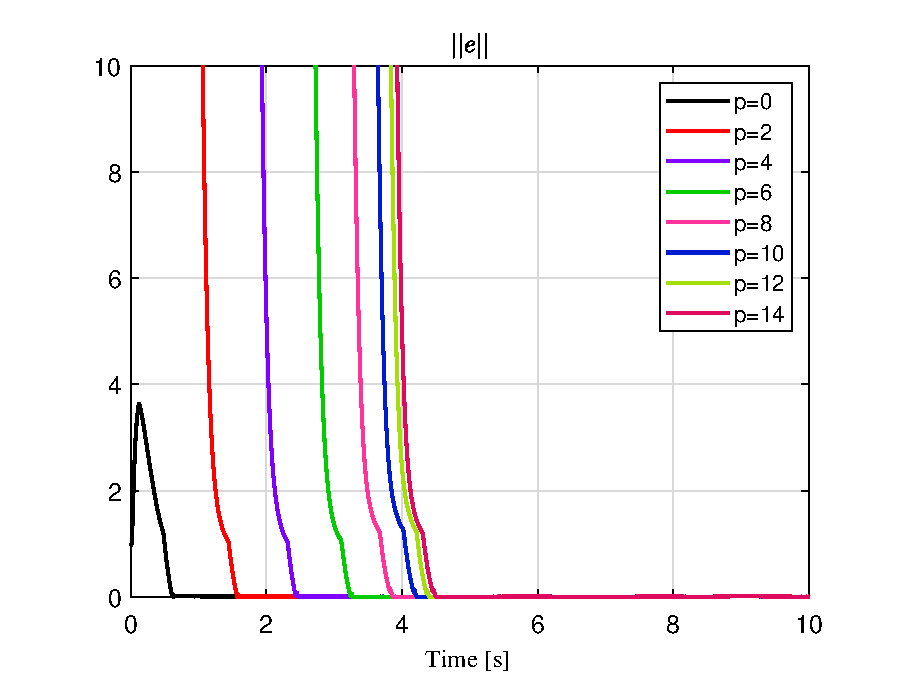
\includegraphics[width=9cm]{sys_4s_disc_FxT_error_orders.eps}}
% 		\caption[SISO HOSM-UIO Fixed-Time estimation]{HOSM-UIO. Estimation error with different orders at initial error $e_0$ showing fixed-time estimation. With $\hat{x}_{0,j}=1\times 10^{p},j=1,...,4$.
% 		}
% 	\label{fig: CH4 Error 4s norm with orders}
% \end{figure}

% \begin{figure}[htbp]
% 	\centering{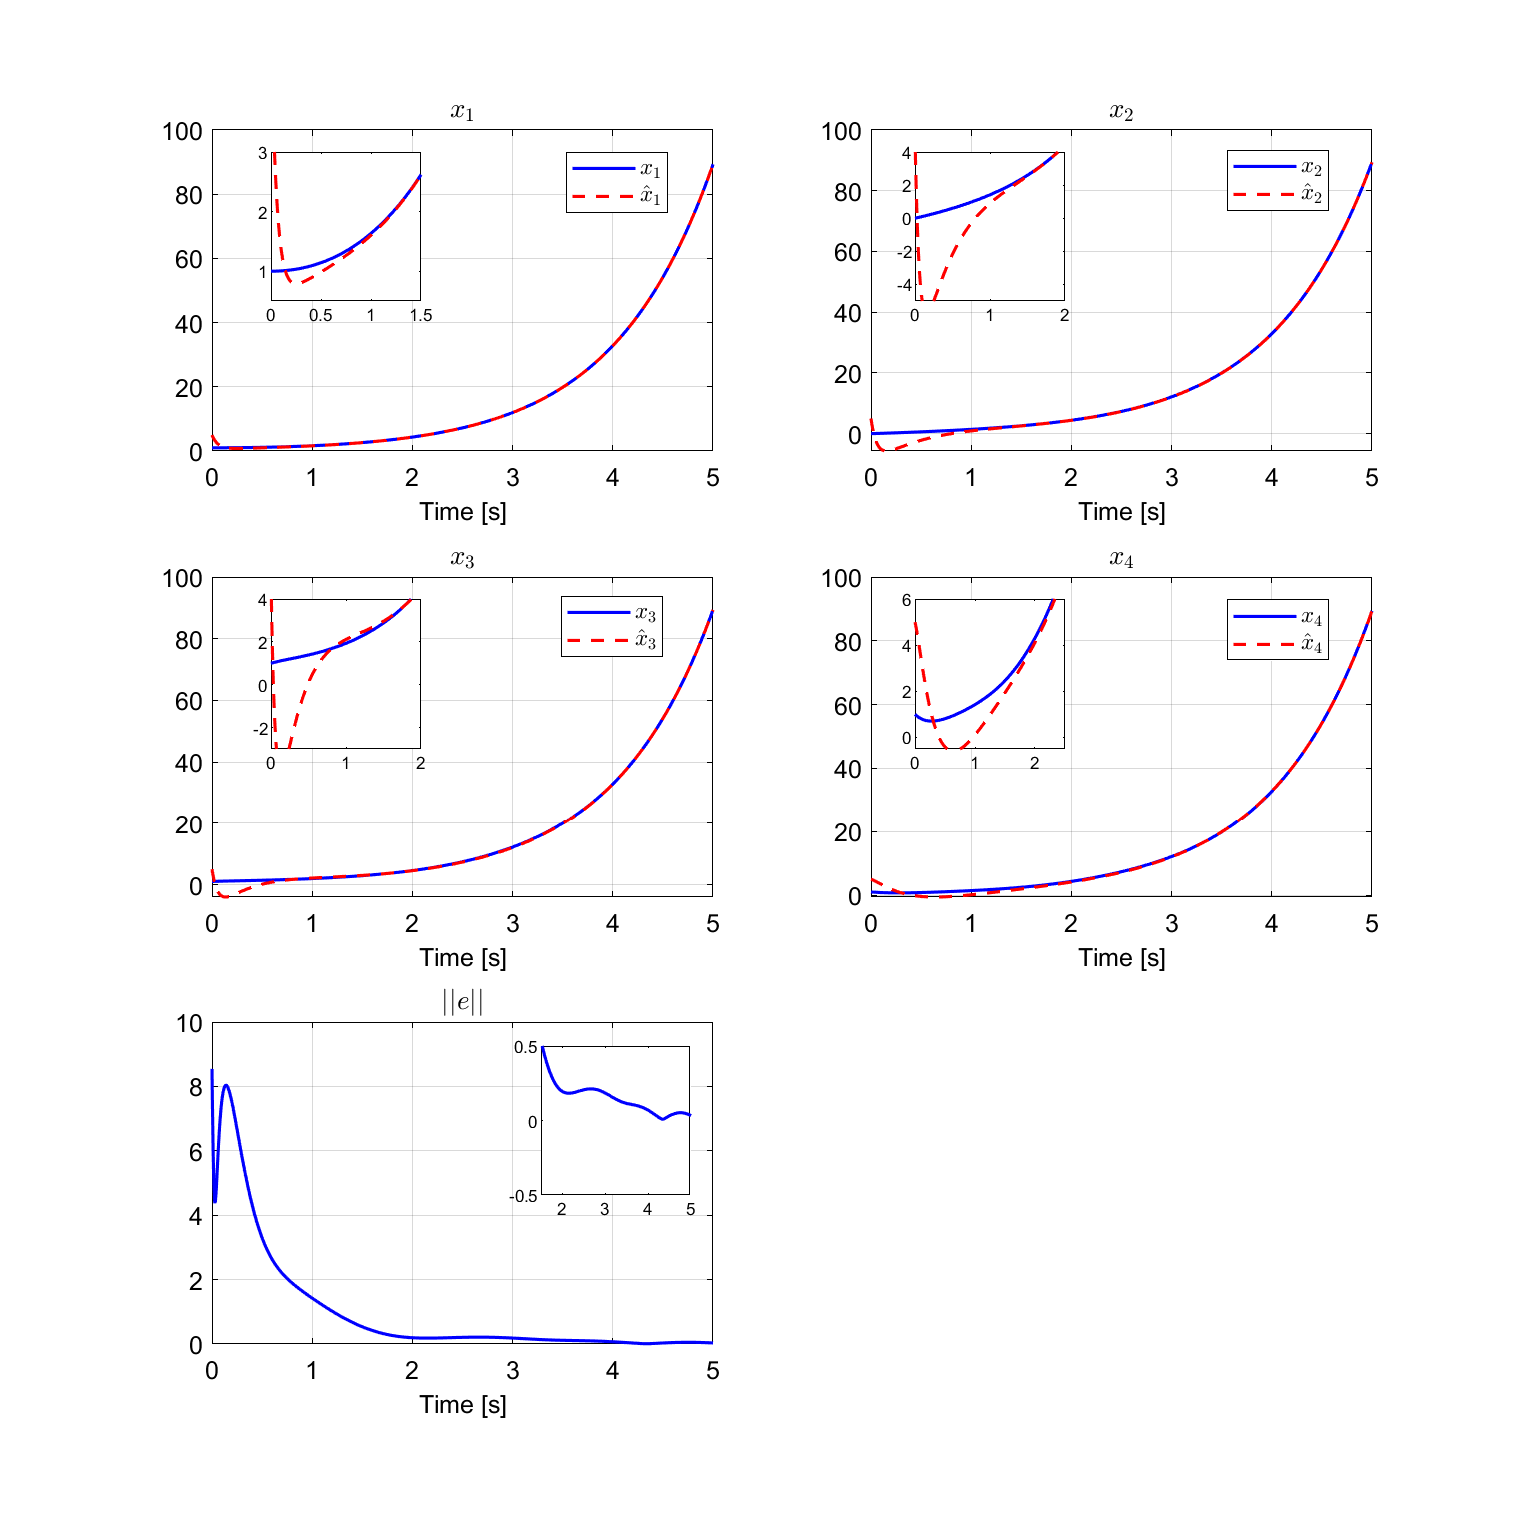
\includegraphics[width=15.8cm]{sys_4s_linear_states.eps}}
% 	\caption[SISO Linear UIO]{Linear UIO. Plant state $x$, state estimation $\hat{x}$ and estimation errors $e=\hat{x}-x$.}
% 	\label{fig: CH4 Error 4s states and norm, e_0 linear}
% \end{figure}

% \begin{figure}[htbp]
% 	\centering{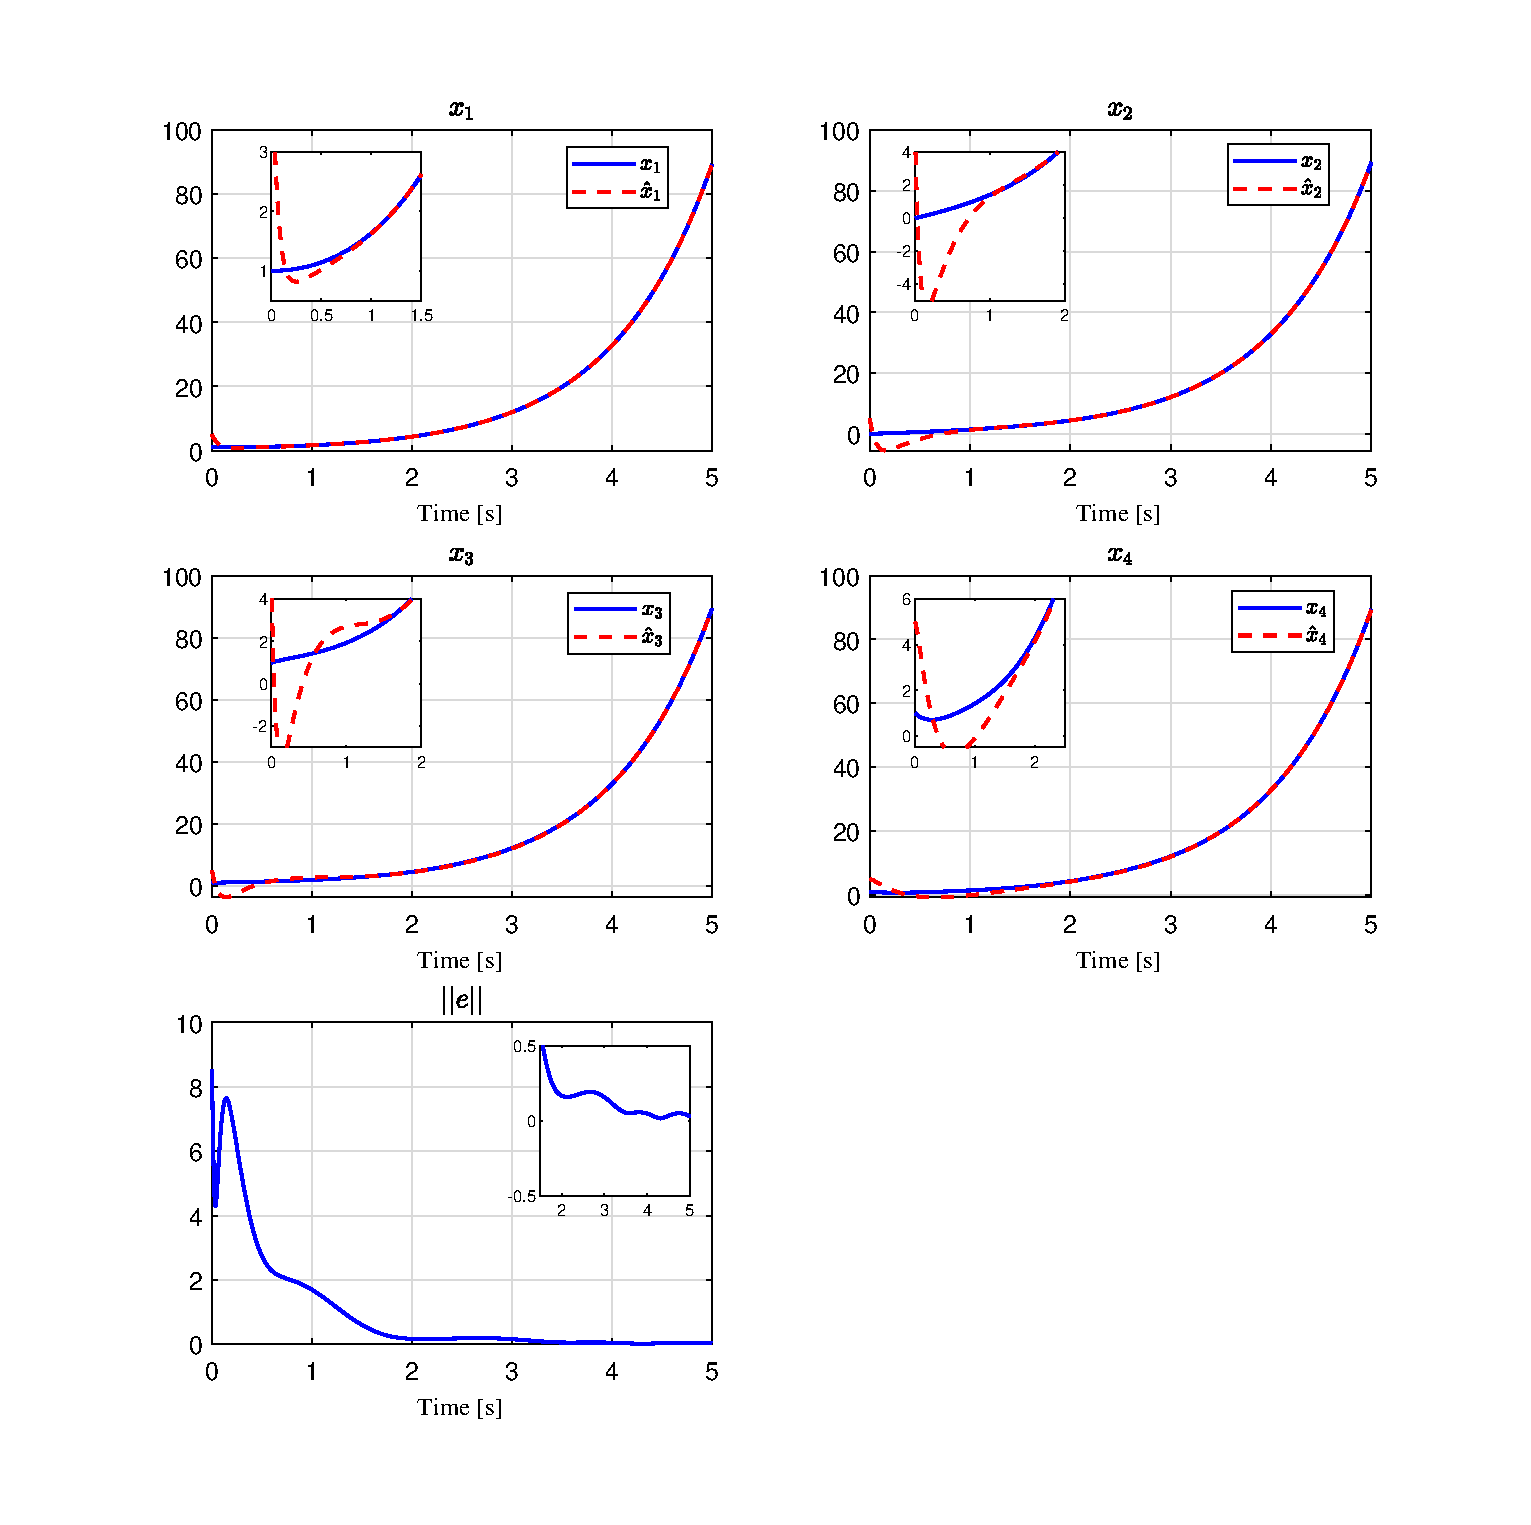
\includegraphics[width=17cm]{sys_4s_cont_states.eps}}
% 	\caption[SISO Continuous UIO]{Continuous UIO. Plant state $x$, state estimation $\hat{x}$ and estimation errors $e=\hat{x}-x$.}
% 	\label{fig: CH4 Error 4s states and norm, e_0 cont}
% \end{figure}

% \begin{figure}[htbp]
% 	\centering{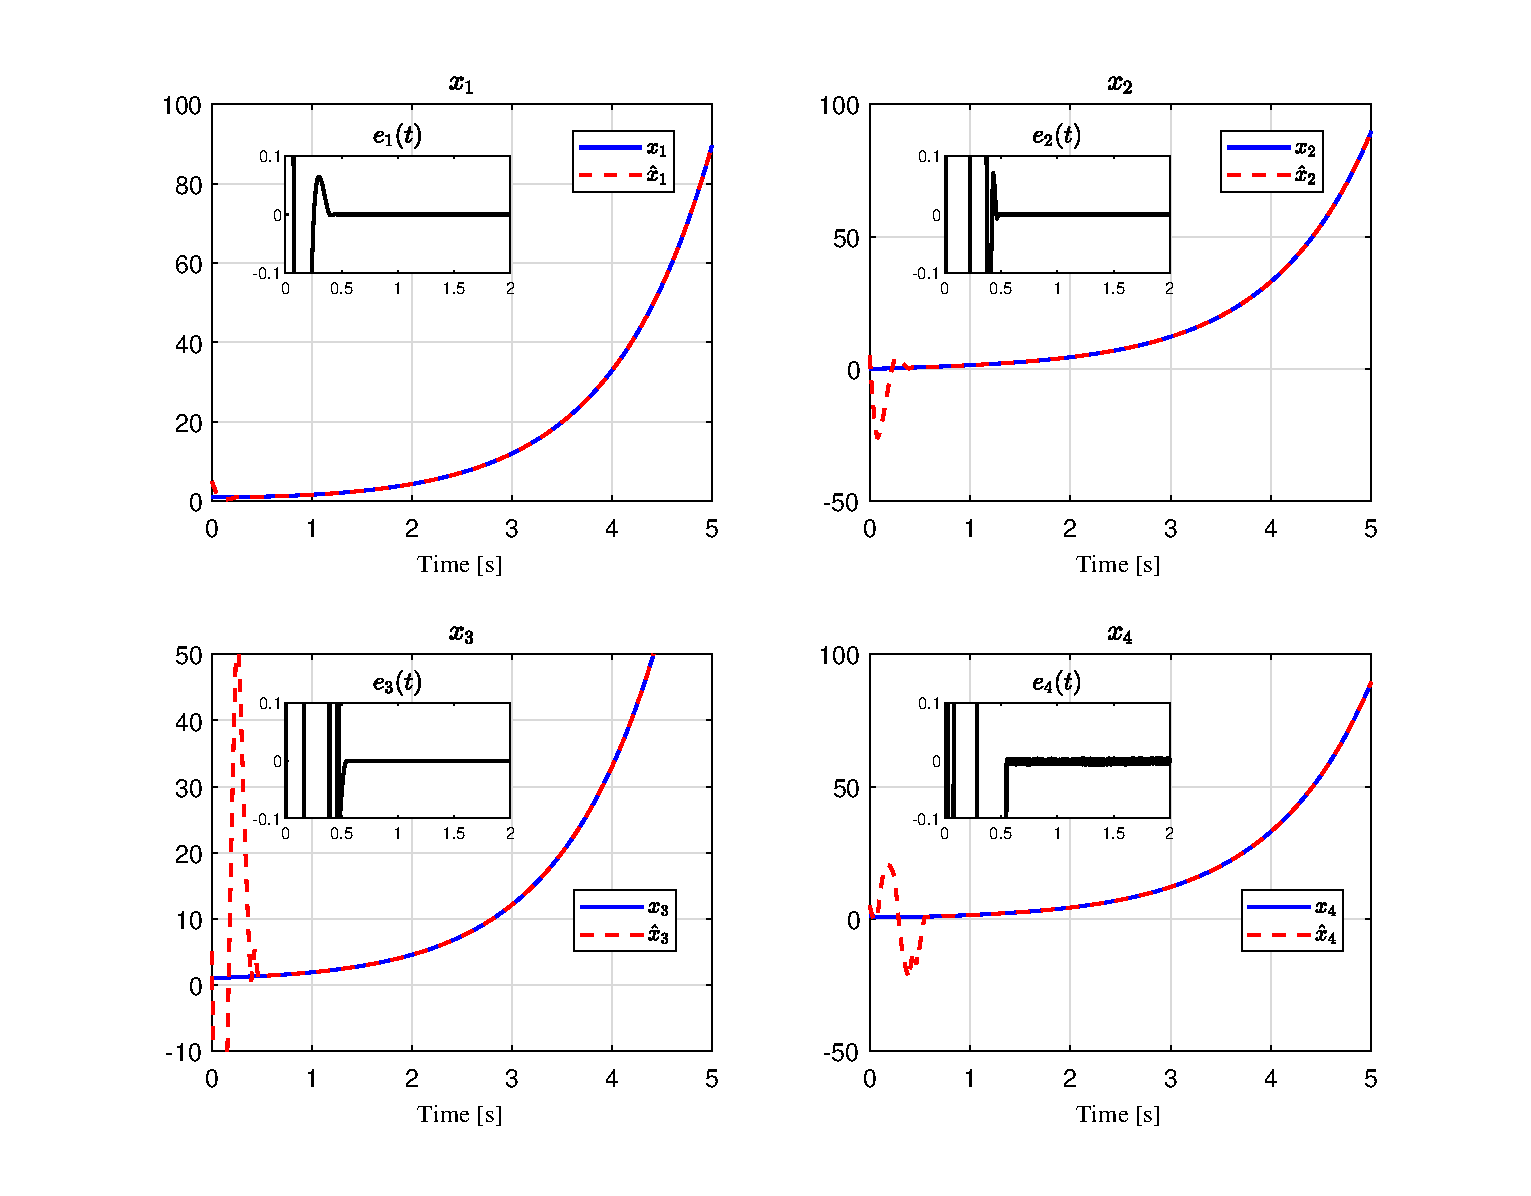
\includegraphics[width=17cm]{sys_4s_disc_states.eps}}
% 	\caption[SISO HOSM-UIO]{HOSM-UIO. Plant state $x$, state estimation $\hat{x}$ and estimation errors $e=\hat{x}-x$.}
% 	\label{fig: CH4 Error 4s states and norm, e_0 disc}
% \end{figure}



